\documentclass[10pt,twocolumn,letterpaper]{article}

\usepackage{cvpr}
\usepackage{times}
\usepackage{epsfig}
\usepackage{graphicx}
\usepackage{amsmath}
\usepackage{amssymb}

% Include other packages here, before hyperref.

% If you comment hyperref and then uncomment it, you should delete
% egpaper.aux before re-running latex.  (Or just hit 'q' on the first latex
% run, let it finish, and you should be clear).
\usepackage[breaklinks=true,bookmarks=false]{hyperref}

\cvprfinalcopy % *** Uncomment this line for the final submission

\def\cvprPaperID{****} % *** Enter the CVPR Paper ID here
\def\httilde{\mbox{\tt\raisebox{-.5ex}{\symbol{126}}}}

% Pages are numbered in submission mode, and unnumbered in camera-ready
%\ifcvprfinal\pagestyle{empty}\fi
\setcounter{page}{1}
\begin{document}

%%%%%%%%% TITLE
\title{Face Matching: Replication of Google Facenet}

\author{Saipranav Janyavula\\
University of Michigan\\
Ann Arbor, MI\\
{\tt\small sjanyavu@umich.edu}
% For a paper whose authors are all at the same institution,
% omit the following lines up until the closing ``}''.
% Additional authors and addresses can be added with ``\and'',
% just like the second author.
% To save space, use either the email address or home page, not both
% \and
% Second Author\\
% Institution2\\
% First line of institution2 address\\
% {\tt\small secondauthor@i2.org}
}

\maketitle
%\thispagestyle{empty}


%%%%%%%%% BODY TEXT
\section{Introduction}
The goal of the project is to create a face matching system that can recognize a person's face and find other pictures of the same person by utilizing the Google Facenet model.
This type of system is quite common and is today part of the default functionality of common photo storage and photo sharing applications and services including Apple Photos, Google Photos, and Amazon Photos.
These applications automatically scan all photos and create albums for each unique person (or even animal) found. Given that this functionality is commercially available (with generally good efficacy), 
there is no practical application to this project. 
It primarily serves as an educational experience and a tool to demonstrate my learning in taking EECS 442.
Combined with a simple user interface, it can serve as a simple and quite visual demonstration that can be shown to others. 
%-------------------------------------------------------------------------

\section{Related Work}
Facenet (2014) was part of the first generation of models which applied Convolutional Neural Networks (CNN's) to the task of Face recognition.
The earliest models (such as Eigenfaces, 1991) utilized various forms of principal component analysis and created vector embeddings representing the combination of base “eigen pictures” that would recreate the original face.
Later methods would continue to build on this work without Neural Networks, with algorithms such as the Discriminant Face Descriptor achieving 80\% accuracy on the Labeled Faces in the Wild (LFW) Dataset.\\

However by utilizing Neural Networks, algorithms such as Facebook's deepface and Google's Facenet would match or exceed human performance on popular datasets such as Labeled Faces in the Wild.\\

Although Facenet and related models represented a big advancement in 2014, facial recognition models have continued to advance since then.
Apple's on-device face recognition model is built on the AirFace face recognition model that utilizes a linear version of the ArcFace angular loss function.
This is then combined with a body embedding model to boost accuracy and reliability. 

\section{Method}
The Facenet paper didn't create a new network architecture.
Instead it modified two previous architectures, one from Zeiler\&Fergus labeled NN1, and the other by C.Szegedy et.al. labeled NN2 which were originally created for image classification.
The minor modifications led to a 128 dimension embedding vector as the output.
These were then trained by utilizing a triplet loss function where each sample consists of 3 images (as embeddings): an anchor, a positive (representing the same identity as the anchor), and a negative(representing a different identity).
The loss function attempts to minimize the difference between the l2 distance from the anchor to the positive, maximize the l2 distance from the anchor to the negative plus a constant margin as shown in the equation below.\\
\begin{equation}
   \sum_{i}^{N} \left[\|f(x_i^a) - f(x_i^p) \|_2^2 - \|f(x_i^a) - f(x_i^n) \|_2^2 + \alpha\right]_+
\end{equation}
The big contribution of the Facenet paper was the utilization of an online triplet selection algorithm.
Traditionally triplets would be pre-generated which could lead to issues as if the negative vector was already very far, the model would learn slowly.
Alternatively if the negative vectors were already very close (and therefore “hard”), it could lead to a local minima in training.
To combat this, the paper generated triplets during training (or “online”) for each batch by generating all possible anchor-positive pairs and selecting a “hard” negative for each.\\

\begin{figure}[t]
   \begin{center}
      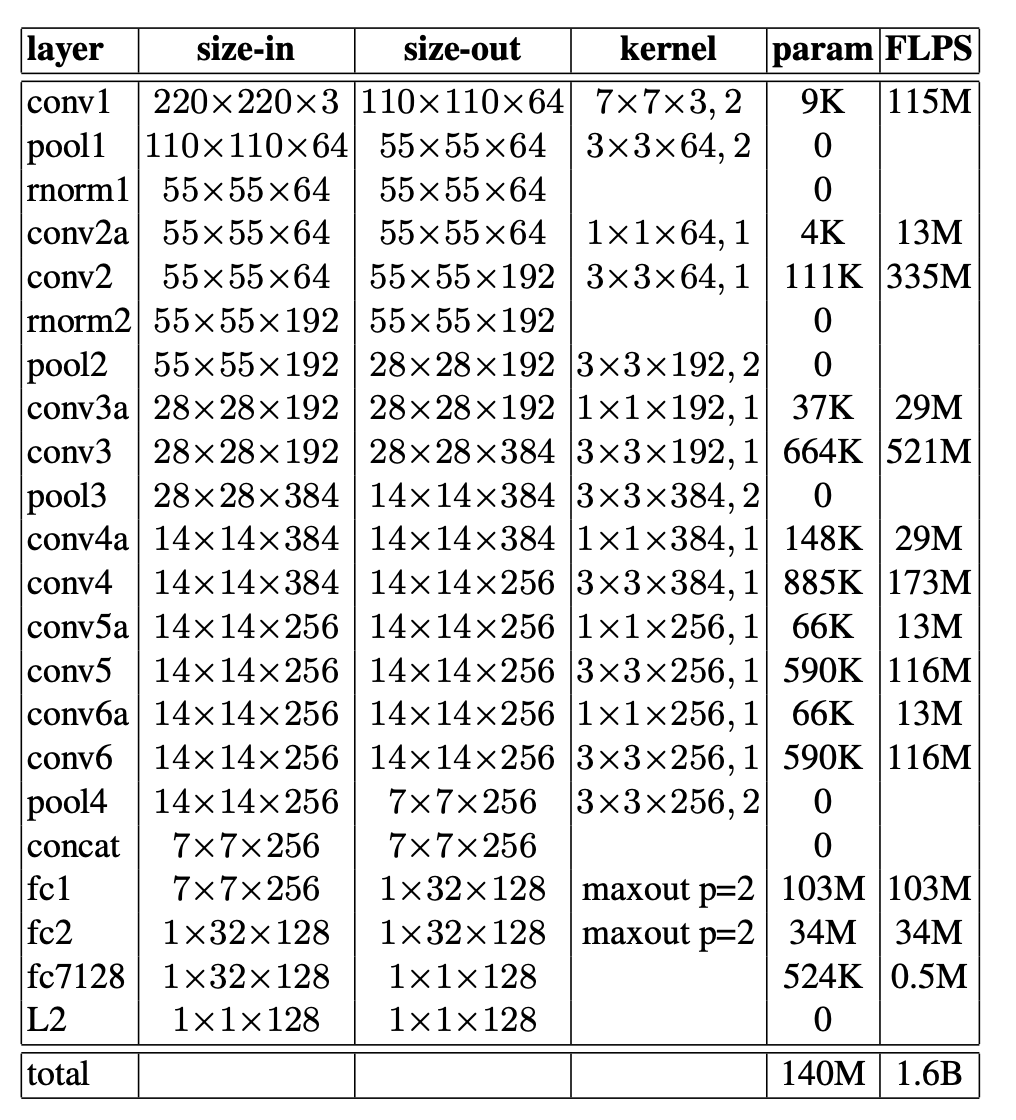
\includegraphics[width=0.8\linewidth]{NN1.png}
   \end{center}
      \caption{NN1 by Zeiler\&Fergus }
   \label{fig:NN1}
   \end{figure}

In their experiments, both NN1 and NN2 (while having different numbers of parameters) both had similar accuracy levels, so I chose to implement NN1 as shown in figure \ref{fig:NN1}.
To do this I replicated all the layers in pytorch except for the “concat” layer as I didn't fully understand what operation was taking place, and added padding as necessary to achieve the same output sizes.
For training data I utilized Microsoft's DigiFace-1M dataset which consists of 1 Million synthetically generated faces.
However due to the comparatively low resolution of these images (112 by 112px), I chose to remove the maxout pooling operations from between the linear layers to prevent a dimensional reduction below 128.
Additionally as I was unable to figure out how to perform effieient triplet selection, I utilized triplet selection code from Adam Bielski's siamese-triplet github repository


\begin{figure*}
   \begin{center}
      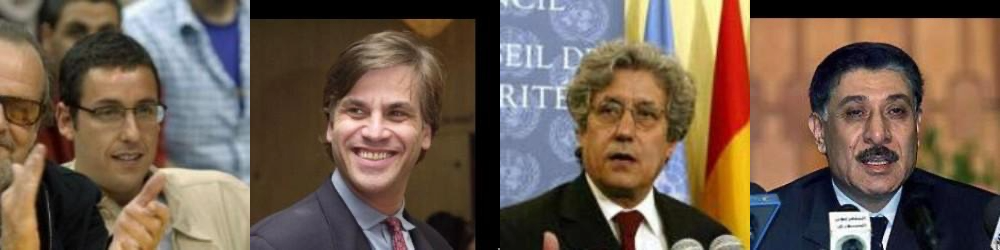
\includegraphics[width=0.8\linewidth]{False Positives.png}
   \end{center}
      \caption{Sample False Positives.}
   \label{fig:falsePositives}
   \end{figure*}

\section{Experiments}
The model was trained on google colab on the v100 gpu.
Due to memory limitations and for speed of training, the batch size was limited to 10 identities with 20 photos per identity.
Across 400 batches, this led to a total training set size of 80k images taking 3.57 hours to complete 50 epochs.\\
This is in contrast to the original paper which utilized between 100M-200M images with 1800 images per batch.
The original paper trained the model on a cpu cluster which ran for between 1000-2000 hours.
For learning parameters, the original paper utilized Adagrad with a triplet loss margin of 0.2 and a learning rate of 0.05.
In my implementation I replicated these parameters except for the learning rate decay which I arbitrarily set at a constant 0.001 as the paper provided no further explanation beyond the statement that they lowered the learning rate to finalize the model.\\

For testing I utilized the LFW dataset by combining all 530 images of George W. Bush (the most of any person in the dataset) with XX images from all people whose names start with the letter A.
As a baseline, I utilized a pretrained model from the facenet\_pytorch library to match images of Bush given a single image of him.
Both models were provided with resized and normalized face snippets from the MTCNN model in the facenet\_pytorch library.
The pretrained model unsurprisingly performed well with a 98.4\% accuracy rate.
Given the same task, my model matched 368 out of 529 images giving it a 69.4\% accuracy rate.
However it also matched 382 out of 1054 negatives giving it a 36.2\% false positive rate as shown in figure \ref{fig:falsePositives}.\\

As a smaller experiment, I attempted to utilize personal photos however the model performed poorly.
Out of 10 personal photos, with 5 containing myself, the model matched 4 images without myself and one image with me where it matched on another person.
This is likely due to the fact that the LFW dataset comprises public (likely professionally taken) images of public figures which would most likely be from various press-conferences or other public events where there is likely to be good lighting and the subject is most likely centered and in focus.
Additionally the LFW images where most likely taken with DSLR cameras which have a depth of field effect not present in most smartphone images unless added digitally.


\section{Conclusion}
\begin{figure}[t]
   \begin{center}
      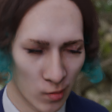
\includegraphics[width=0.8\linewidth]{14.png}
   \end{center}
      \caption{Sample image from DigiFace-1M dataset }
   \label{fig:face}
\end{figure}
As stated earlier, this project has no practical application given the modern prevalence of highly accurate commercial solutions.
As an academic exercise, one can consider many potential improvements to the training of the model including the usage of larger batch sizes with more identities which could enable the selection of better triplets leading to faster training.
There is also likely a data quality issue.
Although the Microsoft DigiFace dataset provided a large number of samples, being digitally generated they are likely to not be fully representative of real images and generally lack the level of detail present in real images.
This can be seen visually in Figure \ref{fig:face} where the synthetic images appear blurry and distorted.
Additionally the images were of a uniform and low resolution of 112x112px compared to Google's dataset which had images across a range of resolutions from 94-244px which would likely prevent the model from overfitting as the images are more varied.
The Facenet paper also provided relatively little information on learning rate decay, experimenting with this will likely lead to improvements as I simply chose an arbitrary constant decay rate of 0.001.\\


However the bigger takeaways are in my opinion personal. This project revealed that I had core misunderstandings about CNN's and Machine Learning in general.
One of the biggest issues was that I didn't understand how to switch from a convolutional layer, with a tensor of shape [batch size, depth, width, height] to a linear layer which requires the tensor to be reshaped into 2d with dimensions [batch size, depth x width x height].
When I first attempted to build the network I simply set the parameters to the desired depth and assumed that pytorch would automatically perform the correct operation.
Similarly I found that I lacked a full understanding of how to vectorize algorithms which led me to utilize pre-written triplett selection code from Adam Bielski's siamese-triplet github repository.
This experience has taught me that there is still a lot more to learn in this field and I anticipate further growth as I continue my educational and professional career.


\section{References}
https://machinelearning.apple.com/research/recognizing-people-photos\\
https://github.com/adambielski/siamese-triplet\\
https://github.com/timesler/facenet-pytorch\\
Facenet: https://arxiv.org/abs/1503.03832\\
Deepface: \begin{verbatim}https://scontent-cgk1-1.xx.fbcdn.net/v/t39.8562-6/240890413_887772915161178_4705912772854439762_n.pdf?_nc_cat=109&ccb=1-7&_nc_sid=e280be&_nc_ohc=aBdItnQKHZ8AX84q8dl&_nc_ht=scontent-cgk1-1.xx&oh=00_AfBDjSTZG9NsOLcNkq2u6z9JGtvFET756lWffW5Ab8I1AA&oe=657FF27F\end{verbatim}
Airface: \begin{verbatim}https://arxiv.org/pdf/1907.12256.pdf\end{verbatim}
Eigenfaces: \begin{verbatim}
https://watermark.silverchair.com/jocn.1991.3.1.71.pdf?token=AQECAHi208BE49Ooan9kkhW_Ercy7Dm3ZL_9Cf3qfKAc485ysgAAA0QwggNABgkqhkiG9w0BBwagggMxMIIDLQIBADCCAyYGCSqGSIb3DQEHATAeBglghkgBZQMEAS4wEQQMUiv3zocAFNGM9C4VAgEQgIIC92e61Fsz2G8f2mUnuskvtgm4l-qfLJqb-1eFNhFOh_Tk5egA-1qsYXguZng6KaBDo8TCCMsYgSe14wxc7FY8ZZQESrGcrMFqBqQh7v3Sy99zEb6E_xxfeLfYgbvNwX7Im1WkQDi_FjB3zu3QExFpMYKdWBA5A0BjZ6IYs9AnWOrTEypl4T8i83XYltBWGyophE2iTO8hu5cOYXOo7e94mAcE_9YyvkB-8Nog3dVb3AY2E-GDoLvyNyQj7lwxTJQL_SoJXp8EcUl80V6heEMsp_PVgdEcGf7kZvxitltNLCNr8S3UhL4uBO59MWMD4sAoDH-xfnemKbFmVE33LpQPrWPehG81DheWoBwIoWYOnNirQDKV-0sSS-nLKUDOujW-KWpp8m-QrcSHJJbKz-G_kjDLTBwYUTd8tXSFUpyANvcaHUBE04lFyGL2yc3fcX4CL5BNJj3KjrGBJyYGTDfLK5xgJDb2weY1FBtybdVnft8SkgZs1YQmZTi73wxTD9xt7YjQf0G17ZQwuj0-FOp13nFfiDaXY3G3oCJ_790PYcTht622DGbMKmLds5Ae4p4bfKaa6AAZxcy3WfdcJGiu2SMzmDFvYy-aUQ8aX7uDCAgv8i5OUMmtLmFibuzaiZvIoJSxyv6Gt2ZLHCYR8JO9jO5krTkqFUqLjZxu5zmu56uIYa9CIMoNK9eZC-DatMdNjjuBH3vh7AHzzYmNzL_KC4GcAtxcFpVH8am-_iwGDTx8YaLLYR_yoy74C39xZomVeQLd_BW9X0pSQtBPHMwEZPDPHdwwtTzh1tf6mHziJJYvtrm9xIlz2L-il_3H0cV8aFWC8O3o1XOaPJkM5rXcobUv9pD6mQSsAQyPqSY0m6IDa7ihZHAjT0g5ff4OaD6z9AgnCg7kx3cNAqQwklKUNGQfpsjK_7OoY9ZWnkA7VEJppGpfbgzevcDgzHmpBnGF52HjI6lPznZ7eX-R784Ixc_VVct6NwgJNts8byB3xDpFrSUA61q7xg
\end{verbatim}
Zieler: \begin{verbatim}
https://arxiv.org/abs/1311.2901
\end{verbatim}
Szegedy: \begin{verbatim} https://arxiv.org/abs/1409.4842 \end{verbatim}
\end{document}